% Capítulo 2. Preparación de Nodos y Entorno de Ejecución (Común a las 3 VPS)
\section{Preparación de Nodos y Entorno de Ejecución (Común a las 3 VPS)}\label{cap:02_preparacion_nodos}
Antes de instalar cualquier componente de la plataforma, las tres VPS se dejan en un mismo estado base: acceso de administración configurado, sistema actualizado, misma zona horaria, Podman instalado y la estructura de carpetas creada con sus permisos. Los pasos de este capítulo se ejecutan en el VPS Frontend (169.58.62.111), el VPS Backend (156.67.26.73) y el VPS Base de Datos (169.58.62.99); cuando un paso aplica solo a uno de ellos, se indica.

% Actualización base y acceso a los servidores
\subsection{Actualización base y acceso a los servidores}\label{sec:2_1_actualizacion_acceso}
Las tres VPS son servidores con Ubuntu 24.04.5 LTS contratados con el proveedor Contabo. La administración se realiza de forma remota por SSH con el cliente Termius, usando la cuenta \texttt{root}. Esta sección explica primero cómo se configura ese acceso y después la actualización del sistema y la zona horaria, que es lo primero que se ejecuta al entrar a cada servidor.

\subsubsection{Acceso por SSH como root con Termius}
\paragraph{Cliente utilizado.} Termius es un cliente SSH gráfico para Windows, macOS y Linux que guarda la lista de servidores con sus credenciales, abre cada conexión en una pestaña o en paneles dentro de un mismo espacio de trabajo (\emph{Workspace}) e incluye un explorador SFTP para transferir archivos. Se utiliza en lugar de la terminal del sistema para tener en un solo lugar las tres VPS de la plataforma y trabajar con ellas al mismo tiempo.

\paragraph{Registro de los servidores.} En Termius se crea un \emph{host} por cada VPS desde \textbf{Hosts $\rightarrow$ New host}, con los siguientes datos:

\begin{table}[H]
\centering
\caption{Hosts registrados en Termius}
\small
\begin{tabular}{llccc}
\toprule
\textbf{Label (nombre)} & \textbf{Address} & \textbf{Puerto SSH} & \textbf{Usuario} & \textbf{Autenticación} \\
\midrule
FRONTEND DEFENSORIA & 169.58.62.111 & 22 & root & Contraseña \\
BACKEND DEFENSORIA & 156.67.26.73 & 22 & root & Contraseña \\
BASE DEFENSORIA & 169.58.62.99 & 22 & root & Contraseña \\
\bottomrule
\end{tabular}
\end{table}

\begin{enumerate}
  \item En \textbf{Address} se escribe la IP pública de la VPS.
  \item En \textbf{General} se asigna el nombre con el que aparecerá en la lista (\emph{Label}).
  \item En \textbf{SSH on port} se deja el puerto \texttt{22}.
  \item En \textbf{Credentials} se captura el usuario \texttt{root} y su contraseña. Termius la guarda cifrada en su bóveda (\emph{vault}) personal, por lo que no es necesario escribirla en cada conexión.
  \item Se guarda el host y se repite para las otras dos VPS.
\end{enumerate}

\begin{figure}[H]
\centering
\begin{subfigure}[t]{0.31\textwidth}\centering
  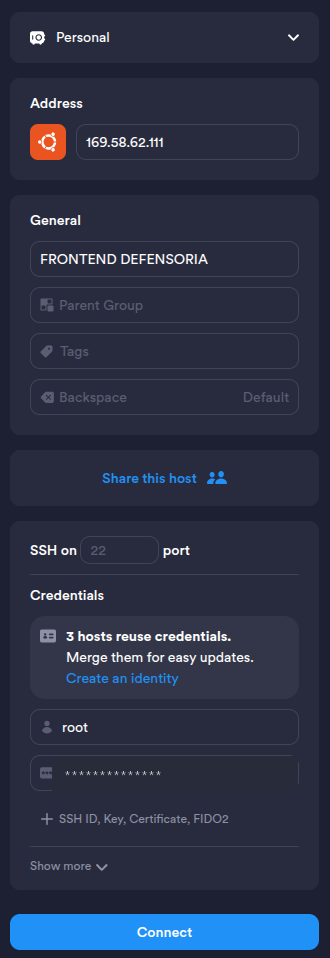
\includegraphics[width=\textwidth]{images/capturas/prep-02-termius-frontend.png}
  \caption{VPS Frontend}
\end{subfigure}\hfill
\begin{subfigure}[t]{0.31\textwidth}\centering
  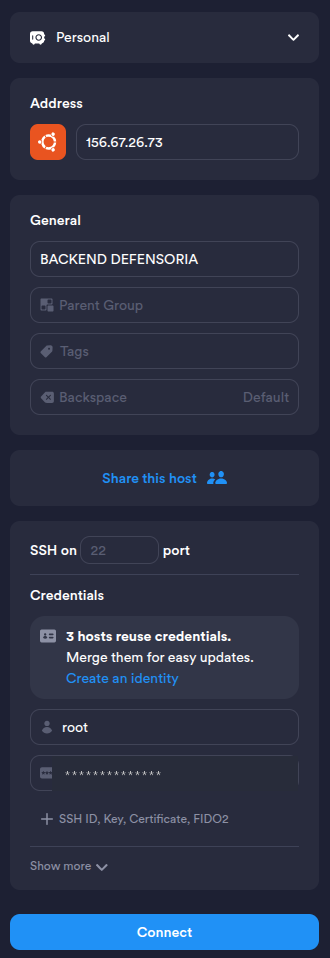
\includegraphics[width=\textwidth]{images/capturas/prep-03-termius-backend.png}
  \caption{VPS Backend}
\end{subfigure}\hfill
\begin{subfigure}[t]{0.31\textwidth}\centering
  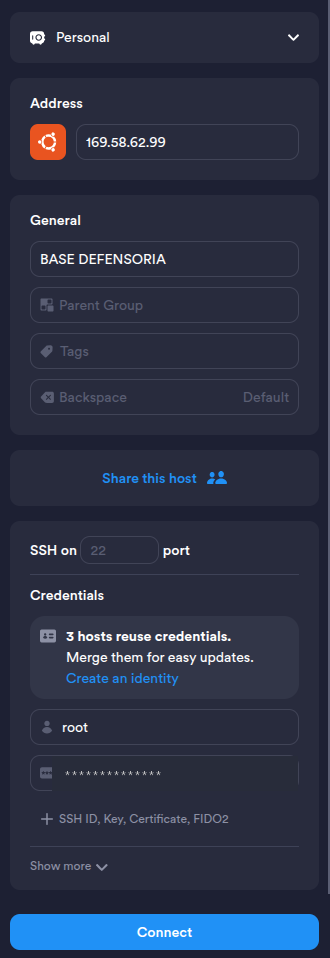
\includegraphics[width=\textwidth]{images/capturas/prep-04-termius-bd.png}
  \caption{VPS Base de Datos}
\end{subfigure}
\caption{Configuración de los tres hosts en Termius (contraseña oculta)}\label{fig:termius-hosts}
\end{figure}

\paragraph{Conexión a las tres VPS.} Al seleccionar un host y pulsar \textbf{Connect}, Termius abre la sesión SSH. En la primera conexión muestra la huella digital (\emph{fingerprint}) de la llave del servidor y pide confirmarla; al aceptarla la registra en \textbf{Known Hosts}. Si en una conexión posterior la huella cambia sin que el servidor se haya reinstalado, se debe rechazar la conexión, porque puede tratarse de un servidor suplantado.

Para la instalación conviene abrir las tres sesiones en un mismo \emph{Workspace}, de modo que las tres VPS quedan visibles a la vez (Figura \ref{fig:prep-05-termius-conexion}). El \emph{prompt} de cada panel muestra el nombre de host del servidor (\texttt{root@vmi3633026}, \texttt{root@vmi3633021}, \texttt{root@vmi3633025}), lo que permite confirmar en qué VPS se está escribiendo antes de ejecutar un comando. La opción \textbf{Broadcast} de Termius envía lo que se escribe a todos los paneles a la vez y sirve para los pasos idénticos en las tres VPS (actualización, zona horaria, instalación de Podman).

\captura{prep-05-termius-conexion}{Sesión SSH como root en las tres VPS dentro de un Workspace de Termius}

\nota{El acceso se hace con usuario \texttt{root} y contraseña, sin llaves SSH. Se recomienda que la contraseña sea larga (16 caracteres o más) y distinta en cada VPS: Termius advierte en la Figura \ref{fig:termius-hosts} que los tres hosts reutilizan las mismas credenciales, de modo que si una se filtra quedan expuestos los tres servidores. Las contraseñas no se escriben en este manual y, al tomar capturas de Termius, el campo de contraseña debe quedar oculto.}

\subsubsection{Actualización del sistema y zona horaria (America/Mexico\_City)}
\paragraph{Actualización de paquetes.} Al conectarse, Ubuntu indica en el mensaje de bienvenida cuántas actualizaciones están pendientes (entre 12 y 14 en la Figura \ref{fig:prep-05-termius-conexion}). En cada VPS se actualiza la lista de paquetes y se instalan:
\begin{lstlisting}
# apt update
# apt upgrade -y
\end{lstlisting}
Si la actualización incluyó un kernel nuevo, Ubuntu crea el archivo \texttt{/var/run/reboot-required}; en ese caso se reinicia la VPS y se vuelve a conectar desde Termius:
\begin{lstlisting}
# [ -f /var/run/reboot-required ] && reboot
\end{lstlisting}

\nota{El mensaje de bienvenida también ofrece actualizar a Ubuntu 26.04 LTS (\texttt{do-release-upgrade}). \textbf{No} se aplica: la plataforma se instaló y probó sobre Ubuntu 24.04 LTS, que sigue recibiendo actualizaciones de seguridad; un cambio de versión mayor se planea por separado.}

\captura{prep-06-apt-upgrade-frontend}{Actualización del sistema en el VPS Frontend}
\captura{prep-07-apt-upgrade-backend}{Actualización del sistema en el VPS Backend}
\captura{prep-08-apt-upgrade-bd}{Actualización del sistema en el VPS Base de Datos}

\paragraph{Zona horaria.} Las VPS vienen con la zona horaria del centro de datos de Contabo en Europa; por eso el mensaje de bienvenida de la Figura \ref{fig:prep-05-termius-conexion} muestra la hora en \texttt{CET}. Se cambian a la hora del centro de México para que las fechas de los registros del sistema, de los logs de los contenedores y de los respaldos coincidan con la hora local de la Defensoría (por ejemplo, el respaldo diario programado a las 4:00 se ejecuta a las 4:00 hora de México y no a media noche):
\begin{lstlisting}
# timedatectl set-timezone America/Mexico_City
# timedatectl
\end{lstlisting}
La salida de \texttt{timedatectl} debe mostrar \texttt{Time zone: America/Mexico\_City (CST, -0600)} y \texttt{System clock synchronized: yes}; esto último indica que el reloj se sincroniza automáticamente por NTP.

\captura{prep-09-zona-horaria-frontend}{Zona horaria America/Mexico\_City en el VPS Frontend}
\captura{prep-10-zona-horaria-backend}{Zona horaria America/Mexico\_City en el VPS Backend}
\captura{prep-11-zona-horaria-bd}{Zona horaria America/Mexico\_City en el VPS Base de Datos}

\nota{La base de datos también trabaja en esta zona horaria: el contenedor \texttt{defensoria-db} se crea con \texttt{TZ=America/Mexico\_City} y el script de inicialización fija la misma zona en \texttt{defensoria\_db} (capítulo \ref{cap:05_despliegue_base_datos}).}

% Instalación y aprovisionamiento de Podman
\subsection{Instalación y aprovisionamiento de Podman}\label{sec:2_2_instalacion_podman}
Todos los componentes de la plataforma (base de datos, microservicios, modelo de IA, frontends y nginx) se ejecutan en contenedores. Como motor de contenedores se usa Podman, que es compatible con las imágenes y los Dockerfile de Docker pero no necesita un proceso servidor (\emph{daemon}) permanente: cada contenedor es un proceso más del sistema, lo que reduce el consumo de memoria en VPS pequeñas.

\subsubsection{Instalación de Podman y utilerías (podman, curl, iptables, python3, certbot)}
En las \textbf{tres} VPS se instalan Podman y las utilerías que usan los scripts de la plataforma:
\begin{lstlisting}
# apt install -y podman curl iptables
# podman --version
\end{lstlisting}
\begin{itemize}
  \item \texttt{podman}: motor de contenedores. Ubuntu 24.04 instala la versión 4.9.
  \item \texttt{curl}: pruebas de los servicios desde la terminal (\texttt{curl http://127.0.0.1:<puerto>}).
  \item \texttt{iptables}: reglas de firewall que aplican los scripts de la plataforma (capítulo \ref{cap:03_seguridad_red_firewall}).
\end{itemize}

Además, según el servidor:
\begin{lstlisting}
# apt install -y python3            # solo VPS Backend
# apt install -y certbot            # solo VPS Frontend
\end{lstlisting}
\begin{itemize}
  \item \texttt{python3} (Backend): lo usa el generador de la carga masiva de quejas (\texttt{generar-csv.py}).
  \item \texttt{certbot} (Frontend): emisión y renovación del certificado HTTPS (sección \ref{sec:7_3_certificados_certbot}).
\end{itemize}

\captura{prep-12-podman-frontend}{Instalación de Podman y versión en el VPS Frontend}
\captura{prep-13-podman-backend}{Instalación de Podman y versión en el VPS Backend}
\captura{prep-14-podman-bd}{Instalación de Podman y versión en el VPS Base de Datos}

\subsubsection{Imágenes base con nombre completo (docker.io/library/...)}
Podman puede buscar una imagen en varios registros cuando se le da un nombre corto (por ejemplo \texttt{postgres}); en ese caso pregunta de forma interactiva de cuál registro descargarla, lo que detiene un script. Para evitarlo, todos los scripts y Dockerfile de la plataforma usan el nombre completo de la imagen, con registro incluido, por lo que no es necesario modificar \texttt{/etc/containers/registries.conf}:

\begin{table}[H]
\centering
\caption{Imágenes base de la plataforma}
\footnotesize
\begin{tabular}{p{8.7cm}p{2.0cm}p{3.6cm}}
\toprule
\textbf{Imagen} & \textbf{VPS} & \textbf{Uso} \\
\midrule
\texttt{docker.io/library/postgres:16-alpine} & Base de datos & \texttt{defensoria-db} \\
\texttt{docker.io/library/eclipse-temurin:21-jre-jammy} & Backend & Microservicios y modelo de IA \\
\texttt{docker.io/library/nginx:alpine} & Frontend & \texttt{router-nginx} y los 5 frontends \\
\bottomrule
\end{tabular}
\end{table}

Para comprobar que la VPS puede descargar imágenes de Docker Hub, se descarga la imagen que le corresponde:
\begin{lstlisting}
# podman pull docker.io/library/nginx:alpine                  # Frontend
# podman pull docker.io/library/eclipse-temurin:21-jre-jammy  # Backend
# podman pull docker.io/library/postgres:16-alpine            # BD
# podman images
\end{lstlisting}
\captura{prep-15-podman-images}{Imagen base descargada en cada VPS (salida de podman images)}

\subsubsection{Contenedores ejecutados como root con podman run}
Los contenedores de la plataforma se crean como \texttt{root} (modo \emph{rootful}) con el comando \texttt{podman run}, que los scripts de cada servidor ejecutan con todos sus parámetros (nombre, puertos, memoria, volúmenes y variables). Se eligió este modo porque:
\begin{itemize}
  \item \texttt{router-nginx} necesita escuchar en los puertos 80 y 443, que en Linux están reservados para \texttt{root}.
  \item Los volúmenes montados (datos de PostgreSQL, configuración, respaldos) pertenecen a \texttt{root}, igual que el resto de \texttt{/apps}.
  \item Todos los contenedores, imágenes y reglas de firewall quedan administrados desde la misma cuenta con la que se conecta Termius.
\end{itemize}
En modo \emph{rootful}, Podman guarda las imágenes y contenedores en \texttt{/var/lib/containers/storage}. Se verifica con:
\begin{lstlisting}
# podman info --format '{{.Store.GraphRoot}}'
# podman ps -a
\end{lstlisting}
La primera línea debe mostrar \texttt{/var/lib/containers/storage}; \texttt{podman ps -a} aparece vacío hasta que se levanten los componentes en los capítulos 5 a 7.

\subsubsection{Arranque automático de contenedores (podman-restart.service)}
Como Podman no tiene un \emph{daemon}, los contenedores no vuelven a arrancar solos después de reiniciar la VPS. Para lograrlo, Podman incluye el servicio de systemd \texttt{podman-restart}, que al encender el servidor levanta todos los contenedores creados con la política \texttt{-{}-restart always}. Se habilita en las tres VPS:
\begin{lstlisting}
# systemctl enable --now podman-restart.service
# systemctl is-enabled podman-restart.service
\end{lstlisting}
La salida debe ser \texttt{enabled}. Los scripts de la plataforma crean cada contenedor con \texttt{-{}-restart always}, por lo que este servicio es el que garantiza que la plataforma se recupere sola tras un reinicio.
\captura{prep-16-podman-restart}{Servicio podman-restart habilitado}

% Estructura de directorios y gestión de permisos
\subsection{Estructura de directorios y gestión de permisos}\label{sec:2_3_directorios_permisos}
Todos los archivos de la plataforma viven bajo \texttt{/apps} en cada VPS. Las carpetas se crean en este paso, vacías y con sus permisos; los archivos (scripts, JAR, configuración, frontends) se colocan en ellas en los capítulos 5 a 7.

\subsubsection{Árbol de carpetas en /apps (aplicaciones/defensoria, data/postgresql, respaldos, utiles/respaldos)}
\begin{table}[H]
\centering
\caption{Carpetas principales}
\small
\begin{tabular}{p{6.2cm}p{8.3cm}}
\toprule
\textbf{Carpeta} & \textbf{Contenido} \\
\midrule
\nolinkurl{/apps/aplicaciones/defensoria} & Scripts, configuración y artefactos de la plataforma (las tres VPS) \\
\nolinkurl{/apps/data/postgresql} & Datos de PostgreSQL (solo VPS Base de Datos) \\
\nolinkurl{/apps/respaldos/bd} & Respaldos de la base generados por \texttt{podman-compose-bd.sh backup} (VPS Base de Datos) \\
\nolinkurl{/apps/utiles/respaldos} & Respaldos generados desde el Panel de la Defensora (VPS Backend) \\
\bottomrule
\end{tabular}
\end{table}

\paragraph{VPS Base de Datos (169.58.62.99).}
\begin{lstlisting}
/apps/
|-- aplicaciones/defensoria/
|   |-- database/              podman-compose-bd.sh
|   `-- database-scripts/
|       |-- init/              00-init.sql (se ejecuta al crear la base)
|       `-- seeds/             01..05-*.sql (datos semilla)
|-- data/postgresql/           defensoria_db/ (la crea el script)
`-- respaldos/bd/              respaldos .sql.gz
\end{lstlisting}

\paragraph{VPS Backend (156.67.26.73).}
\begin{lstlisting}
/apps/
|-- aplicaciones/defensoria/back/
|   |-- Dockerfile, podman-compose.sh, podman-compose-modelo.sh, firewall-backend.sh
|   |-- artifact/              11 archivos .jar
|   |-- admin-service/         Dockerfile propio de admin-service
|   |-- config-files/          <servicio>/config/<servicio>.yml
|   |-- modelo/Dataset/        corpus JSON del modelo de IA
|   |-- modelo/pruebas/        peticiones de prueba del modelo
|   `-- carga-masiva/          cargar-quejas.sh, generar-csv.py
`-- utiles/respaldos/          respaldos del Panel de la Defensora
\end{lstlisting}

\paragraph{VPS Frontend (169.58.62.111).}
\begin{lstlisting}
/apps/aplicaciones/defensoria/
|-- front/                     defensoria-web (portal)
|   |-- config/                static.conf
|   `-- dist/browser/          archivos compilados de Angular
|-- front-admin/dist/browser/            admin-web
|-- front-revision/dist/browser/         revision-web
|-- front-primer-contacto/dist/browser/  primer-contacto-web
|-- front-subdefensoria/dist/browser/    subdefensoria-web
`-- router/
    |-- config/                defensoria.conf (router-nginx)
    `-- certbot-webroot/       reto HTTP-01 de Let's Encrypt
\end{lstlisting}

\paragraph{Creación de las carpetas.} En el VPS Base de Datos:
\begin{lstlisting}
# A=/apps/aplicaciones/defensoria
# mkdir -p $A/database $A/database-scripts/init $A/database-scripts/seeds \
           /apps/data/postgresql /apps/respaldos/bd
\end{lstlisting}
En el VPS Backend:
\begin{lstlisting}
# B=/apps/aplicaciones/defensoria/back
# mkdir -p $B/artifact $B/admin-service $B/config-files \
           $B/modelo/Dataset $B/modelo/pruebas $B/carga-masiva \
           /apps/utiles/respaldos
\end{lstlisting}
En el VPS Frontend:
\begin{lstlisting}
# F=/apps/aplicaciones/defensoria
# mkdir -p $F/front/config $F/front/dist/browser \
           $F/front-admin/dist/browser $F/front-revision/dist/browser \
           $F/front-primer-contacto/dist/browser $F/front-subdefensoria/dist/browser \
           $F/router/config $F/router/certbot-webroot
\end{lstlisting}

\subsubsection{Políticas de propiedad y permisos (root:root, 755 carpetas, 750 scripts, 750/640 config-files, 700 respaldos)}
Todo \texttt{/apps} pertenece a \texttt{root:root}, porque los contenedores se ejecutan como \texttt{root} (sección \ref{sec:2_2_instalacion_podman}). Los permisos se asignan según lo que contiene cada carpeta o archivo:

\begin{table}[H]
\centering
\caption{Política de permisos}
\small
\begin{tabular}{p{5.4cm}cp{7.2cm}}
\toprule
\textbf{Carpeta o archivo} & \textbf{Permiso} & \textbf{Motivo} \\
\midrule
Carpetas generales & 755 & Cualquiera puede recorrerlas y leerlas; solo \texttt{root} escribe \\
Scripts \texttt{.sh} & 750 & Solo \texttt{root} los ejecuta \\
\texttt{config-files/} (carpetas / archivos) & 750 / 640 & Contienen la contraseña de la BD, el secreto JWT y la contraseña SMTP \\
\texttt{podman-compose-bd.sh} y su carpeta & 700 & El script contiene la contraseña de PostgreSQL \\
JAR, Dockerfile, SQL, JSON, archivos web & 644 & Solo lectura; se copian dentro de las imágenes \\
Carpetas de respaldos & 700 & Contienen copias completas de la base de datos \\
\texttt{database-scripts/init} & 755 / 644 & PostgreSQL ejecuta \texttt{00-init.sql} con su propio usuario dentro del contenedor y necesita leerlo \\
\nolinkurl{/apps/data/postgresql/*} & -- & No se modifica a mano: el contenedor asigna su propio dueño a la carpeta de datos \\
\bottomrule
\end{tabular}
\end{table}

En el VPS Base de Datos:
\begin{lstlisting}
# chown -R root:root /apps
# chmod 755 /apps /apps/aplicaciones /apps/aplicaciones/defensoria /apps/data /apps/data/postgresql
# chmod 755 $A/database-scripts $A/database-scripts/init $A/database-scripts/seeds
# chmod 700 $A/database
# chmod 755 /apps/respaldos && chmod 700 /apps/respaldos/bd
\end{lstlisting}
En el VPS Backend:
\begin{lstlisting}
# chown -R root:root /apps
# chmod 755 /apps /apps/aplicaciones /apps/aplicaciones/defensoria $B \
            $B/artifact $B/admin-service $B/modelo $B/modelo/Dataset \
            $B/modelo/pruebas $B/carga-masiva /apps/utiles
# chmod 750 $B/config-files
# chmod 700 /apps/utiles/respaldos
\end{lstlisting}
En el VPS Frontend:
\begin{lstlisting}
# chown -R root:root /apps
# find /apps -type d -exec chmod 755 {} +
\end{lstlisting}
Los permisos de los archivos (750 para scripts, 640 para configuración, 644 para el resto) se aplican cuando se colocan en los capítulos 5 a 7.

\paragraph{Verificación.} En cada VPS se listan las carpetas con su dueño y permisos:
\begin{lstlisting}
# find /apps -type d -printf "%M %u %g %p\n"
\end{lstlisting}
La salida muestra, por cada carpeta, sus permisos (\texttt{\%M}, por ejemplo \texttt{drwxr-xr-x} = 755), su dueño (\texttt{\%u}), su grupo (\texttt{\%g}) y su ruta (\texttt{\%p}). Cada carpeta debe aparecer con dueño \texttt{root root} y con el permiso de la tabla anterior.
\captura{prep-17-permisos-frontend}{Dueño y permisos de las carpetas en el VPS Frontend}
\captura{prep-18-permisos-backend}{Dueño y permisos de las carpetas en el VPS Backend}
\captura{prep-19-permisos-bd}{Dueño y permisos de las carpetas en el VPS Base de Datos}

